\newcommand*{\pth}{$p^{H}_{\text{T}}$\xspace}
\newcommand*{\htautau}{$H \to \tau \tau$\xspace}
\newcommand*{\ztautau}{$Z \to \tau \tau$\xspace}
\newcommand*{\pt}{$p_{\text{T}}$\xspace}
\newcommand*{\taul}{$\tau$-lepton\xspace}
\newcommand*{\tauhadvis}{\ensuremath{\tauhad}\xspace}
\newcommand*{\mmc}{\ensuremath{m^\text{MMC}_{\tau\tau}}\xspace}
\newcommand*{\taulephad}{$\tau_{\text{lep}}\tau_{\text{had}}$\xspace}
\newcommand*{\tauhadhad}{$\tau_{\text{had}}\tau_{\text{had}}$\xspace}



This chapter presents the core analysis developed in the context of this thesis, focusing on the study of the Higgs boson decay into a pair of $\tau$-leptons produced in association with top-quark pairs. The \( H \to \tau_{\text{had}}\tau_{\text{had}}\) final state is of particular importance, both because of its experimental challenges and because it provides unique sensitivity to the top-Higgs Yukawa interaction. The following sections describe the motivation behind this measurement, the general and specific strategy pursued in ATLAS, the definition of physics objects and event selection, and the improvements introduced during this work with respect to earlier iterations of the analysis. Special emphasis is given to the implementation of multivariate techniques (MVA) for event categorization and to the transition from Run-2 to Run-3 datasets, which mark the evolution of the current measurement program.


%%%%%%%%%%%%%%%%%%%%%%%%%%%%%%%%%%%%%%%%%%%%%%%%%%%%%%%%%%%%%%%%%%%%%%%%%%%%%%%%%%%%%%%%%%%%%%%%%%%%%%%%%%%%%%%%%%%%%%%%%%%%%%%%%%%%%%%%%%%%%%%%%%%%%%%%%%%%%%%%%%%%%%%%%%%%%%%%%%%%
\section{Motivation}
\label{sec:analysis_motivation}

The production of the Higgs boson in association with a top-quark pair provides a privileged way to probe the Yukawa coupling between the two particles, $y_{t}$, since the production cross-section of this process is proportional to the square of this coupling, as already discussed in Section~\ref{sec:ttH}. A direct measurement of this parameter is of particular importance both for confirming the properties of the Higgs boson within the SM and for exploring the nature of the electroweak symmetry breaking mechanism and potential effects beyond the Standard Model (BSM).

As previously mentioned, the $t\bar{t}H$ production mode was first established by ATLAS and CMS in 2018, combining the Higgs boson decays $H \to VV^{*}$, $H \to \tau\tau$, $H \to b\bar{b}$, and $H \to \gamma\gamma$, as illustrated in Figure~\ref{fig:tth_obs}. The results were obtained in terms of the signal strength, $\mu_{t\bar{t}H}$, with an observed excess of $6.3\sigma$ above the SM expectation in ATLAS and $5.2\sigma$ in CMS.

\begin{figure}[htbp]
    \centering
    \begin{subfigure}[b]{0.48\textwidth}
        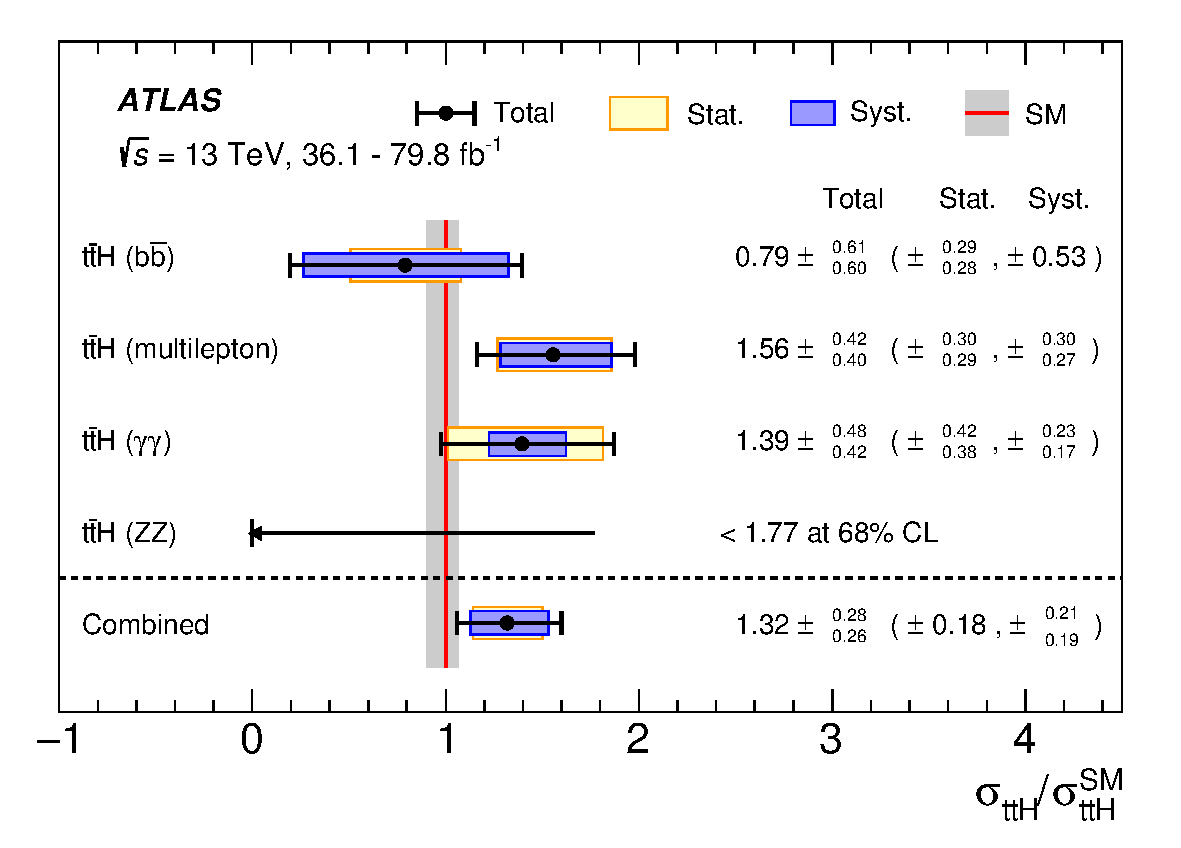
\includegraphics[width=\textwidth]{desv_atlas}
        \caption{}
    \end{subfigure}
    \hfill
    \begin{subfigure}[b]{0.48\textwidth}
        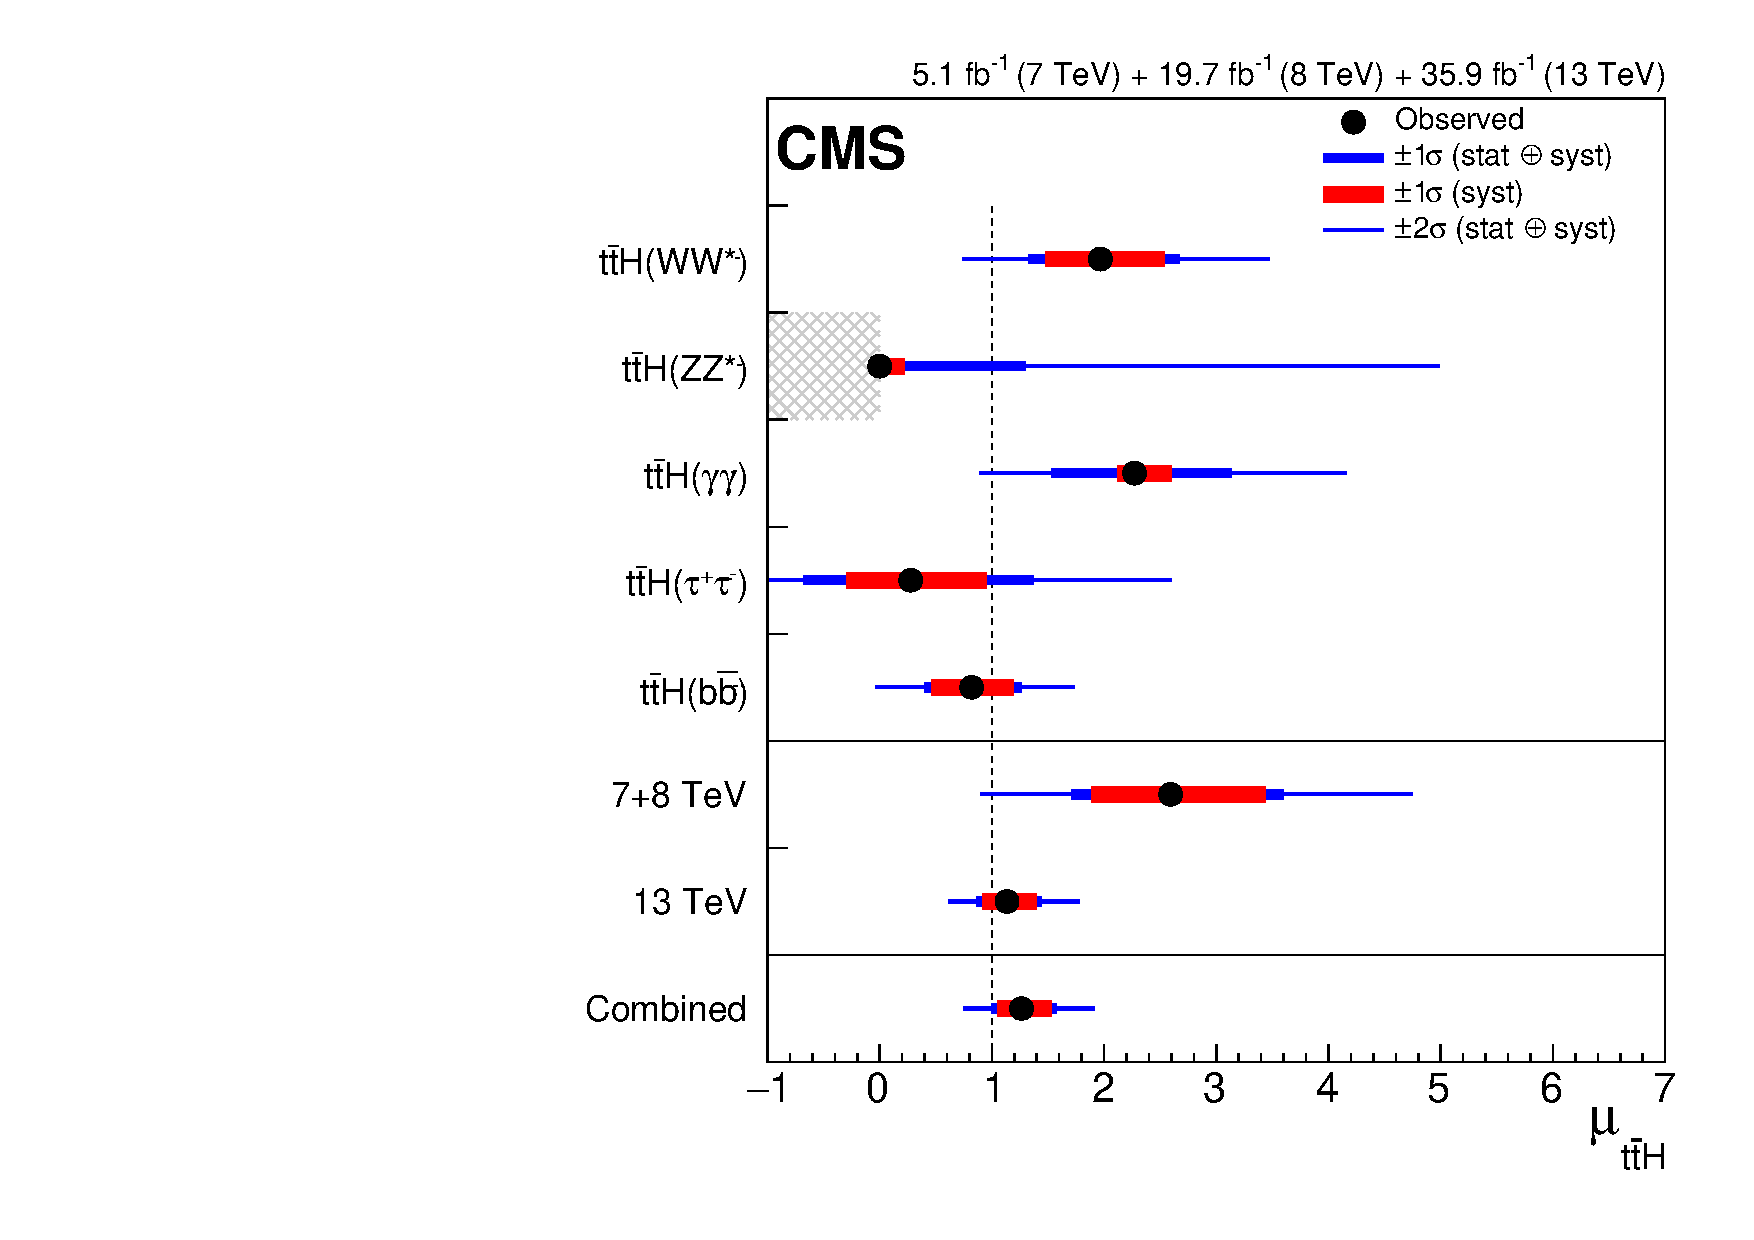
\includegraphics[width=\textwidth]{desv_cms}
        \caption{}
    \end{subfigure}
    \hfill
    \caption{(a) Combined $t\bar{t}H$ production cross-section together with the individual ATLAS measurements, shown as ratios to the SM prediction~\cite{ATLAS:2018mme}. Black lines represent the total uncertainties, while the bands indicate the statistical and systematic components. (b) Best-fit value of the signal strength $\mu_{t\bar{t}H}$ measured by CMS, including the one- and two-standard-deviation confidence intervals~\cite{CMS:2018uxb}.}
    \label{fig:tth_obs}
  \end{figure}

  The \ttH production mode contributes only about 1\% to the total effective Higgs boson production cross-section at the LHC, as indicated in Section~\ref{sec:higgs_production}, with a predicted value of $0.507^{+5.8}_{-9.2} \text{ (QCD scale)} \pm 3.6 \text{ (PDF}+\alpha_{s})$~pb~\cite{https://doi.org/10.23731/cyrm-2017-002}. For this reason, the design of a \ttH analysis requires a careful balance between selecting a decay channel with a sufficiently large branching ratio and ensuring good control over the different background contributions.  

  Following the observation of this production mode, subsequent analyses using the Run-2 dataset focused on improving the precision of the measured cross-section by targeting specific regions of phase space and exploiting decay modes that either maximize sensitivity to the signal or provide enhanced sensitivity to possible BSM effects, either individually or in combination with other Higgs production modes. Among the possible decay channels, $H \to b\bar{b}$ appears particularly attractive due to its large Higgs boson branching ratio. However, \ttH analyses in this channel are strongly affected by the overwhelming background from $t\bar{t}b\bar{b}$ production, which is both large and difficult to model and constrain~\cite{Aad:2904447}.  
  
  In this thesis, the \htautau decay channel is considered as it offers a balanced compromise between signal yield and background control. Moreover, the reconstruction of the di-$\tau$ system in \htautau events provides additional discrimination power against the dominant backgrounds. As already mentioned, the \ttH analysis with \htautau decays is not grouped together with other multilepton final states, but instead constitutes a dedicated category within the broader \htautau analysis, restricted to the case where both $\tau$-leptons decay hadronically. The remaining $\tau$-decay channels are covered by other ATLAS studies~\cite{PhysRevD.97.072003}.  
  
  The first evidence for the \htautau decay channel was established during Run~1. ATLAS reported a significance of $4.5\sigma$~\cite{htau_2015}, and the combination of ATLAS and CMS confirmed the channel with a significance of $5.5\sigma$~\cite{htau_cms_atlas_2016}. Subsequently, Run-2 analyses concentrated on more precise measurements of the total cross-section as well as on the individual contributions of the main production modes. Differential measurements based on kinematic observables such as the transverse momentum of the Higgs boson (\pth) or the jet multiplicity were also performed, as described in Section~\ref{sec:stxs_yukawa}.  
  
  Among the four main Higgs boson production modes, \htautau has provided the most precise results for the $VBF$ production mode. The measurement obtained in the first study using the full Run-2 dataset yielded a cross-section of $0.90^{+0.20}_{-0.17}$ times the SM prediction~\cite{2022}, in good agreement with the CMS result of $0.81 \pm 0.17$ times the SM expectation~\cite{Tumasyan_2023}. For \ttH production, the precision was more limited, but still provided sensitivity, with an inclusive measured production cross-section of $1.06^{+1.28}_{-1.08}$ times the SM prediction. These results were originally derived within the STXS framework, with granularity adapted in \pth, the dijet invariant mass ($m_{\text{jj}}$), and jet multiplicity, resulting in a total of nine fiducial STXS bins: six targeting $ggF$ production and three devoted to $VBF$, $VH$, and \ttH, respectively, as shown in Figure~\ref{fig:atlas_htautau_stxs}.
  
\begin{figure}[htbp]
    \centering
    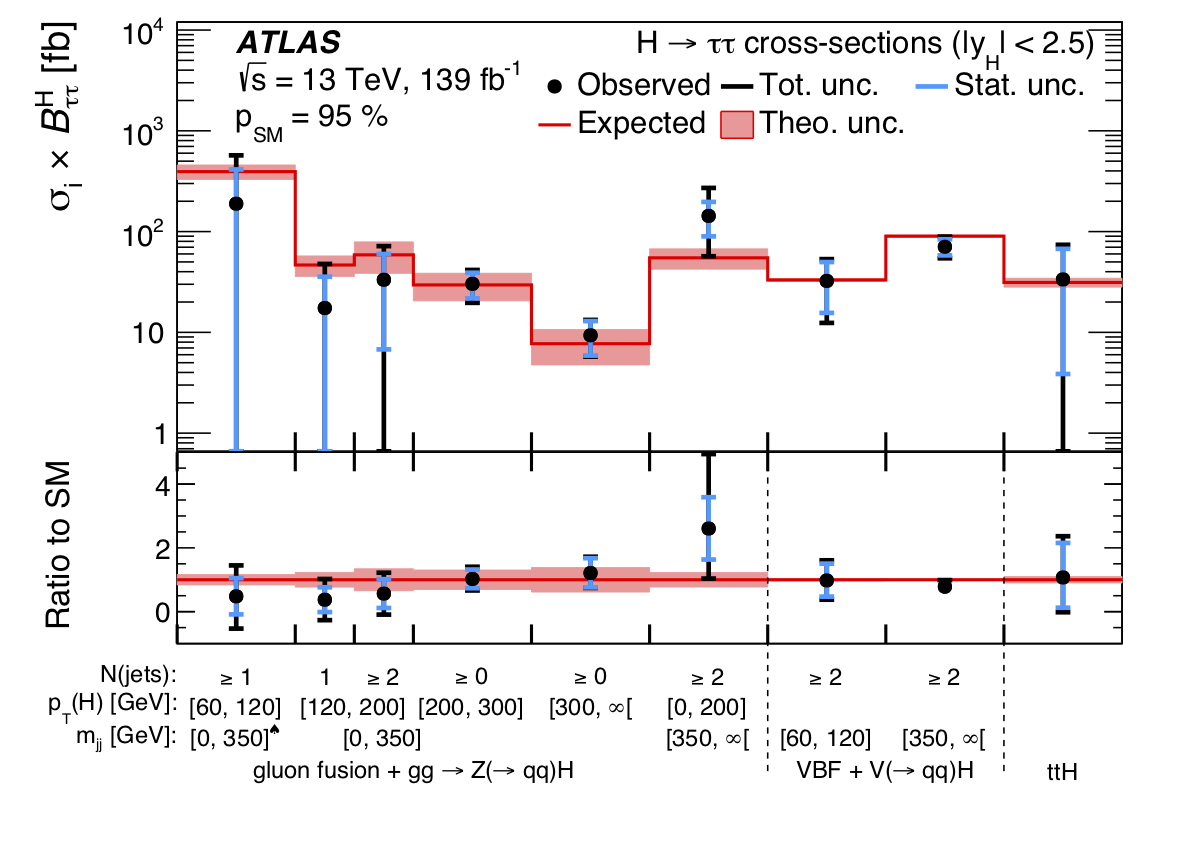
\includegraphics[width=0.7\textwidth]{images/pois_9pois.png}
    \caption{Measured values of $\sigma \times \mathcal{B}(H \to \tau\tau)$ in the nine fiducial regions defined by the STXS framework, from the first ATLAS analysis of $H \to \tau\tau$ using the full Run~2 dataset. Black (blue) error bars represent the total (statistical) uncertainties, while the continuous lines correspond to the SM predictions~\cite{2022}.}
    \label{fig:atlas_htautau_stxs}
\end{figure}

This chapter presents the measurements obtained in the most recent published iteration of the \htautau analysis using the full Run-2 dataset. This new round extends the scope of the STXS results from the previous analysis, including additional STXS bins for the two Higgs boson production modes already mentioned.  

In particular, this thesis focuses on the extension of the \ttH analysis within this framework, moving from an inclusive measurement in the fully hadronic final state to the determination of the cross-section in three separate STXS bins in \pth. This strategy potentially increases the sensitivity to deviations from the SM in the high-\pt\ regions.  

Moreover, a more precise measurement of the $t\bar{t}H(H\to\tau\tau)$ channel is of particular importance in the context of the global and combined Higgs boson measurements performed at ATLAS, where all accessible production and decay modes are simultaneously fitted. In these combinations, significant (anti)correlations have been observed between $t\bar{t}H(H\to\tau\tau)$ and other channels, most notably $t\bar{t}H(H\to WW^*)$, with values reaching up to $-0.45$ in Run-2 fits~\cite{Aad_2020_combined}. Such correlations reduce the overall sensitivity of the combined analyses and limit the ability to disentangle the different Higgs boson production and decay modes. The most recent ATLAS results~\cite{Nature_ATLAS} confirm this effect, with updated correlation coefficients of about $-0.32$ between the $H\to\tau\tau$ and $H\to WW^*$ channels in the global signal strength fits.

%%%%%%%%%%%%%%%%%%%%%%%%%%%%%%%%%%%%%%%%%%%%%%%%%%%%%%%%%%%%%%%%%%%%%%%%%%%%%%%%%%%%%%%%%%%%%%%%%%%%%%%%%%%%%%%%%%%%%%%%%%%%%%%%%%%%%%%%%%%%%%%%%%%%%%%%%%%%%%%%%%%%%%%%%%%%%%%%%%%%

\section{Analysis strategy}
\label{sec:analysis_strategy}

The new measurements presented in this thesis are obtained from the analysis of the full Run-2 dataset, corresponding to an integrated luminosity of $140~\text{fb}^{-1}$ at a centre-of-mass energy of $\sqrt{s}=13$~TeV. Although it is a promising channel, \htautau also presents a number of challenges. The final state can be obscured by certain background processes, most notably \ztautau, which has a cross-section much larger than that of the Higgs boson, and whose mass peak lies not far from the Higgs boson resonance.  

In addition, while the presence of $\tau$-leptons allows for a good reconstruction of the Higgs boson, it must be taken into account that $\tau$-leptons decay before reaching the detector. The resulting final states are therefore complex, containing neutrinos that escape detection. This complicates the reconstruction of the Higgs boson mass and \pt compared with other cleaner channels such as $H \to \gamma\gamma$.  

Another difficulty arises from the fact that certain reconstructed objects can be misidentified as $\tau$-leptons, which must be carefully controlled. The following sections describe the strategy developed to address these issues in this analysis, focusing on the \ttH production mode. At the global level, within the \htautau analysis, events are first categorised according to the decay modes of the $\tau$-leptons into three channels: $\tau_{e}\tau_{\mu}$, $\tau_{\text{lep}}\tau_{\text{had}}$, and $\tau_{\text{had}}\tau_{\text{had}}$. Channels with two electrons or two muons are excluded from the analysis due to their much smaller branching ratios and sensitivity, as they are heavily contaminated by $Z \to \ell\ell$ decays.  

As already mentioned, in \ttHtt only the $\tau_{\text{had}}\tau_{\text{had}}$ final state is considered. In this channel, the dominant background is \ztautau, followed by processes where hadronic $\tau$ decays are misidentified (referred to as ``Fakes''), in which jets are reconstructed as $\tau_{\text{had}}$ candidates. The $Z+$jets background is estimated with MC simulations and normalised to collision data, while the fake background is derived with data-driven techniques to reduce the dependence on simulations. The \ttH channel also suffers from large backgrounds originating from \ttbar events, which are considered in cases with zero, one, or two $\tau_{\text{had}}$, the latter being the dominant contribution. Additional smaller backgrounds include $t\bar{t}V$ and diboson production. These processes are estimated from MC simulations, with the \ttbar background normalised to data, as is the case for \Ztautau.  

The cross-section measurements are performed within the STXS framework, requiring the definition of signal regions targeting the different bins of Stage~1.2 of the STXS strategy. In this new round of the \htautau analysis, the six $ggF$ and the $VH$ bins measured in the previous iteration are retained. The $t\bar{t}H$ production mode is now probed in three $p_{\text{T}}^H$ bins, while VBF production is studied in eight kinematic regions defined by $p_{\text{T}}^H$ and $m_{jj}$. Multivariate analysis techniques are employed in the $VH$, $t\bar{t}H$, and VBF signal regions to enhance the sensitivity to the $H \to \tau\tau$ signal. In addition, inclusive measurements of the total cross-section times branching ratio for $H \to \tau\tau$, as well as of the production-mode cross-sections, are performed.  

The following sections will therefore focus on the new strategy for event categorisation in the \ttH channel using MVA techniques, culminating with the presentation of the results obtained in this new round of the \ttHtt analysis. A general overview of the remaining measurements, including the other production modes in the \htautau analysis, will also be presented, summarising the legacy results of the ATLAS collaboration for this decay channel using the full Run-2 dataset. All results are published in Ref.~\cite{differential_htautau}.

%%%%%%%%%%%%%%%%%%%%%%%%%%%%%%%%%%%%%%%%%%%%%%%%%%%%%%%%%%%%%%%%%%%%%%%%%%%%%%%%%%%%%%%%%%%%%%%%%%%%%%%%%%%%%%%%%%%%%%%%%%%%%%%%%%%%%%%%%%%%%%%%%%%%%%%%%%%%%%%%%%%%%%%%%%%%%%%%%%%%
\section{Object definition and trigger selection}
\label{sec:object_definiton}

As a standard procedure, the selection of candidate events in this analysis relies on the reconstruction and identification of the main physics objects in the detector: electrons, muons, hadronically decaying $\tau$-leptons, jets, and missing transverse momentum. Based on the number and type of these objects, events can be classified into different final states. The analysis presented here focuses exclusively on the $\tau_{\text{had}}\tau_{\text{had}}$ channel, where both $\tau$-leptons decay hadronically, producing narrow hadronic jets together with neutrinos.  

In the following discussion, electrons and muons appearing in the final state will be collectively referred to as light leptons ($\ell$).

\subsection{Trigger criteria}
\label{subsec:trigger_tth}

The first step in defining the events of interest for the analysis is the selection of the triggers to be applied. The corresponding trigger efficiencies in MC are corrected to match those observed in data using scale factors.  

In the $\tau_{\text{had}}\tau_{\text{had}}$ channel, di-tau triggers are employed. The two $\tau_{\text{had-vis}}$ candidates reconstructed offline are required to match the corresponding legs of the online di-tau trigger objects, with $\Delta R > 0.6$. The transverse momentum thresholds are chosen to ensure that the selected $\tau_{\text{had}}$ candidates lie within the trigger efficiency plateau. Specifically, the leading $\tau_{\text{had}}$ candidate must satisfy an online (offline) requirement of $p_{\text{T}} > 35~(40)$~GeV, while the subleading one must exceed $p_{\text{T}} > 25~(30)$~GeV.  

Due to the increased instantaneous luminosity during the 2016--2018 data-taking period, an additional Level-1 calorimeter jet trigger with $p_{\text{T}} > 25$~GeV and $|\eta| < 3.2$ was introduced. To guarantee that the trigger operates consistently within its efficiency plateau, the leading jet in the event is required to have $p_{\text{T}} > 70$~GeV and $|\eta| < 3.2$. The impact of this condition on the signal efficiency has been verified to be below $0.3\%$.

\subsection{Physics objects definition}
\label{subsec:trigger_tth}

The procedure followed for the reconstruction and identification of the physics objects used in this analysis closely follows what has already been described in Chapter~\ref{chap:object_rec}.  
In the \ttHtt analysis, only jets with \pt$>20$~GeV are considered. The JVT is applied to jets with \pt$ > 60$~GeV and $|\eta| < 2.5$ in order to suppress those not associated with the primary vertex, while for jets with \pt$ > 60$~GeV in the forward region ($|\eta| > 2.5$) the fJVT is applied. In the $t\bar{t}H(\tau_{\text{had}}\tau_{\text{had}})$ process, the most relevant jets, such as $b$-jets from the top-quark decays and the $\tau_{\text{had}}$ candidates, are predominantly located in the central region of the detector. This is in contrast to processes such as VBF, where the characteristic signature involves forward jets, while in $t\bar{t}H$ the event topology is mainly central. Figure~\ref{fig:tth_topo} shows two examples of tree-level Feynman diagrams for the \ttHtt process.
\begin{figure}[htbp]
    \centering
    \begin{subfigure}[b]{0.48\textwidth}
        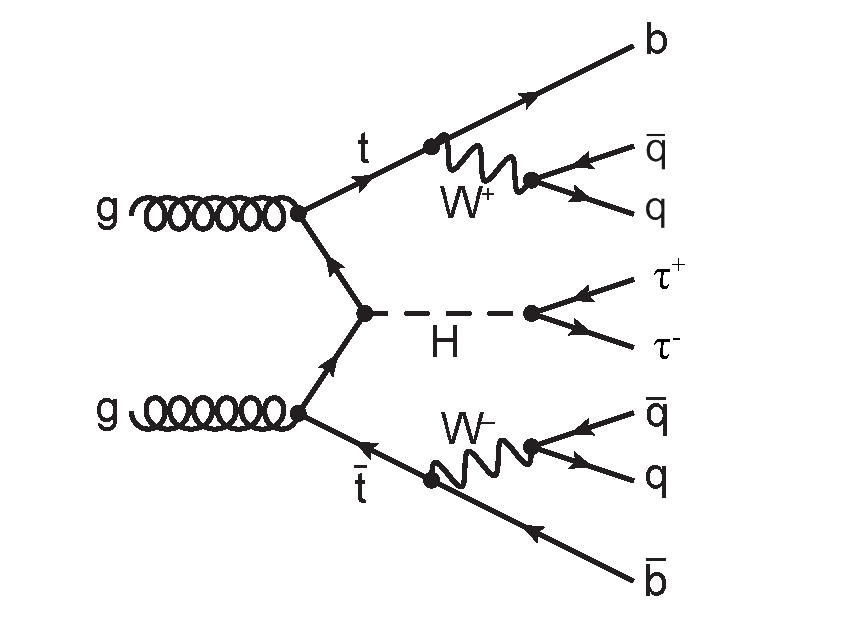
\includegraphics[width=\textwidth]{tth_diagram_1}
    \end{subfigure}
    \hfill
    \begin{subfigure}[b]{0.48\textwidth}
        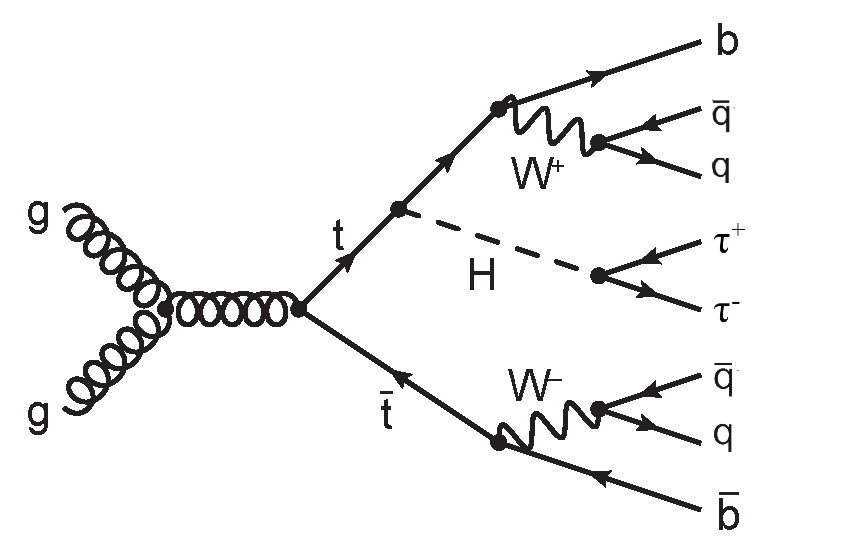
\includegraphics[width=\textwidth]{tth_diagram_2}
    \end{subfigure}
    \hfill
    \caption{Example of tree level diagrams for the \ttHtt process considered in this analyisis.}
    \label{fig:tth_topo}
\end{figure}
\FloatBarrier
The $b$-tagged jets are identified using the DL1r algorithm in this Run-2 release~21 analysis, with a working point corresponding to a fixed efficiency of $70\%$.  

Referring to $\tau_{\text{had-vis}}$ as the detectable products of hadronic $\tau$ decays, the selected $\tau_{\text{had-vis}}$ candidates are required to have \pt$ > 20$~GeV and $|\eta| < 2.47$, excluding the transition region between the barrel and end-cap calorimeters. The charge of the $\tau_{\text{had-vis}}$ candidates is computed as the sum of the charges of the associated tracks, and is required to be $\pm 1$. Candidates are further classified as 1-prong or 3-prong, depending on the number of associated tracks. As discussed in Section~\ref{sec:tauhad}, the same RNN is employed to discriminate $\tau_{\text{had-vis}}$ from quark- or gluon-initiated jets, while the dedicated eBDT is used to suppress electrons misidentified as $\tau_{\text{had-vis}}$. For this analysis, the Medium identification working point is adopted, providing efficiencies of about $75\%$ and $60\%$ for 1-prong and 3-prong $\tau_{\text{had-vis}}$, respectively.  

Finally, the missing transverse momentum, \etmiss, in the events considered for this study is reconstructed as defined in Section~\ref{sec:met}.

%%%%%%%%%%%%%%%%%%%%%%%%%%%%%%%%%%%%%%%%%%%%%%%%%%%%%%%%%%%%%%%%%%%%%%%%%%%%%%%%%%%%%%%%%%%%%%%%%%%%%%%%%%%%%%%%%%%%%%%%%%%%%%%%%%%%%%%%%%%%%%%%%%%%%%%%%%%%%%%%%%%%%%%%%%%%%%%%%%%%
\section{Higgs boson reconstruction}
\label{sec:higgs_reconstruction}

A crucial ingredient of the \htautau analysis, and in particular for $t\bar{t}H(\tau_{\text{had}}\tau_{\text{had}})$, is the reconstruction of the Higgs boson system from the two $\tau$-leptons. In particular, the invariant mass and the transverse momentum of the di-$\tau$ system are the key observables exploited throughout the analysis. The invariant mass serves as the primary handle to discriminate the Higgs boson signal from the dominant irreducible background $Z\to\tau\tau$, as well as from reducible contributions such as $t\bar{t}$ events with misidentified $\tau_{\text{had}}$ candidates. 

\subsection{Higgs boson mass reconstruction}
\label{subsec:higgs_mass}

Since each $\tau$-lepton decay involves one or more neutrinos that escape detection, the full invariant mass cannot be reconstructed directly, and dedicated algorithms are required. In this analysis two approaches are employed: the collinear approximation and the Missing Mass Calculator (MMC).  

The collinear approximation assumes that the neutrinos are emitted in the same direction as the visible $\tau$-lepton decay products. Under this hypothesis, the missing transverse momentum is entirely attributed to the neutrinos, and the momentum fractions $x_1$ and $x_2$ carried by each \taul's visible decay products can be expressed as: 
\begin{align}
    x_{1} &= 
    \frac{p_{x,2}^{\text{vis}} p_{y,1}^{\text{vis}} - p_{y,2}^{\text{vis}} p_{x,1}^{\text{vis}}}
         {p_{x,2}^{\text{vis}} p_{y,1}^{\text{vis}} - p_{y,2}^{\text{vis}} p_{x,1}^{\text{vis}} 
          + E_{x}^{\text{miss}} p_{y,1}^{\text{vis}} - E_{y}^{\text{miss}} p_{x,1}^{\text{vis}}}, \nonumber \\[8pt]
    x_{2} &= 
    \frac{p_{x,2}^{\text{vis}} p_{y,1}^{\text{vis}} - p_{y,2}^{\text{vis}} p_{x,1}^{\text{vis}}}
         {p_{x,2}^{\text{vis}} p_{y,1}^{\text{vis}} - p_{y,2}^{\text{vis}} p_{x,1}^{\text{vis}} 
          - E_{x}^{\text{miss}} p_{y,2}^{\text{vis}} + E_{y}^{\text{miss}} p_{x,2}^{\text{vis}}}.
    \end{align}
being the x and y subscripts the cartesian components of the missing tranverse momentum in the transverse plane. Once the momentum fractions are determined from there, the reconstructed collinear di-$\tau$ mass is
\begin{equation}
m_{\tau\tau}^{\text{coll}} = \frac{m_{\text{vis}}}{\sqrt{x_{1}x_{2}}},
\label{eq:mcoll}
\end{equation}
where $m_{\text{vis}}$ is the visible invariant mass of the two $\tau_{\text{had-vis}}$ candidates, obtained considering only the visible decay products of the \taul. This method provides reasonable resolution in boosted topologies, but can yield unphysical solutions or large overestimates when the collinearity assumption is not valid.  

The Missing Mass Calculator (MMC)~\cite{Elagin_2011} is a more advanced approach designed to overcome the limitations of the collinear approximation. It aims to reconstruct the most probable kinematic configuration of the full di-$\tau$ system, including the invisible neutrinos, by maximizing a likelihood function built from probability density functions derived from $\tau$-decay kinematics. In this framework, six to eight unknown parameters are required to fully describe the event, depending on the $\tau$-lepton decay mode. These variables include the components of the invisible neutrino momenta $\vec{p}^{\,\text{miss}}_{1(2)}$ from each $\tau$ decay, as well as the invariant mass of the invisible system $m^{\text{miss}}_{1(2)}$ for each leptonically decaying $\tau$-lepton. The estimation of these quantities relies on the following mass-shell constraints:

\begin{align}
E_x^{\text{miss}} &= p_1^{\text{miss}} \sin \theta^{\text{miss}}_1 \cos \phi^{\text{miss}}_1 + p_2^{\text{miss}} \sin \theta^{\text{miss}}_2 \cos \phi^{\text{miss}}_2 , \nonumber \\
E_y^{\text{miss}} &= p_1^{\text{miss}} \sin \theta^{\text{miss}}_1 \sin \phi^{\text{miss}}_1 + p_2^{\text{miss}} \sin \theta^{\text{miss}}_2 \sin \phi^{\text{miss}}_2 , \nonumber \\
m_{\tau_1}^2 &= \left(m_1^{\text{miss}}\right)^2 + \left(m_1^{\text{vis}}\right)^2 + 2 E_1^{\text{vis}} E_1^{\text{miss}}
- 2 p_1^{\text{vis}} p_1^{\text{miss}} \cos\left(\theta_1^{\text{vis}} - \theta_1^{\text{miss}}\right) ,  \nonumber \\
m_{\tau_2}^2 &= \left(m_2^{\text{miss}}\right)^2 + \left(m_2^{\text{vis}}\right)^2 + 2 E_2^{\text{vis}} E_2^{\text{miss}}
- 2 p_2^{\text{vis}} p_2^{\text{miss}} \cos\left(\theta_2^{\text{vis}} - \theta_2^{\text{miss}}\right) .
\end{align}
Here, $E^{\text{vis}}_{1(2)}$ and $p^{\text{vis}}_{1(2)}$ denote the energies and momenta of the visible $\tau$-decay products, $m^{\text{vis}}_{1(2)}$ their invariant masses, and $m^{\text{miss}}_{1(2)}$ the invariant mass of the neutrino system. The polar (azimuthal) angles of the visible and invisible decay products are given by $\theta^{\text{vis}}_{1(2)}$ ($\phi^{\text{vis}}_{1(2)}$) and $\theta^{\text{miss}}_{1(2)}$ ($\phi^{\text{miss}}_{1(2)}$), respectively. For hadronically decaying $\tau$-leptons, only one neutrino is produced, so $m^{\text{miss}}_{1(2)}$ is set to zero.  

Even with the above mass-shell constraints, the system remains underdetermined. The MMC addresses this by employing probability density functions derived from $\tau$-decay kinematics, estimated from Monte Carlo simulations. The algorithm scans over the unknown neutrino parameters and selects the most probable configuration by maximizing a likelihood. To mitigate the impact of the resolution of the missing transverse momentum \etmiss, additional scans over $E_x^{\text{miss}}$ and $E_y^{\text{miss}}$ are performed, with each point weighted according to a Gaussian probability based on the calorimeter’s transverse energy sum.  

The MMC provides different estimators of the di-$\tau$ mass, namely the maximum weight (MAXW), the most likely mass (MLM), and the most likely neutrino momenta (MLNU3P), all obtained through Markov Chain Monte Carlo sampling. Among these, the MLM~\cite{mlm_thesis} method is adopted as the nominal choice, as it defines the reconstructed di-$\tau$ mass from the maximum of the likelihood-weighted histogram of sampled points, yielding the most stable estimate across a wide range of topologies.  

The MMC fails to converge in a small fraction of events (about $1\%$ for the $\tau_{\text{had}}\tau_{\text{had}}$ channel). To avoid losing these events, the $m_{\tau\tau}^{\text{coll}}$ mass from Eq.~(\ref{eq:mcoll}) is used as a fallback. In this way, the MMC–MLM serves as the primary invariant mass estimator throughout the analysis, ensuring both accuracy and completeness of the event sample.  

\subsection{Reconstruction of \pth}
\label{subsec:higgs_mass}

In the $H \to \tau\tau$ analysis, the transverse momentum of the Higgs boson, $p_{\text{T}}^H$, plays a central role in the categorization of events within the STXS framework. Traditionally, this observable was reconstructed the four-momenta of the visible $\tau$-leptons together with the \etmiss.

In this analysis, a novel neural network (NN) regression is employed to enhance the reconstruction of $p_{\text{T}}^H$. The NN is trained on simulated Higgs events and uses four input variables: the angular separation $\Delta R_{\tau\tau}$, the azimuthal angle difference $\Delta \phi_{\tau\tau}$ between the two $\tau$-leptons, the transverse momentum of the system formed by their four-momenta and \etmiss, and the collinear mass $m_{\tau\tau}^{\text{coll}}$. Although the network is trained using ggF production events, it can be directly applied to the $t\bar{t}H(\tau_{\text{had}}\tau_{\text{had}})$ channel or other production modes like VBF without requiring retraining, while still yielding a significant improvement in resolution compared to the traditional method.
This enhancement can be directly observed in Figure~\ref{fig:ptH_resolution}, where the resolution of both reconstruction methods is compared in VBF-produced Higgs boson events. The distribution is significantly narrower, yielding an improvement of approximately $50\%$.

The improved reconstruction of $p_{\text{T}}^H$ reduces bin-to-bin migrations in the STXS framework, thereby providing a more faithful mapping between reconstructed and truth-level distributions. This improvement is particularly exploited in the design of the MVA strategy used to discriminate $t\bar{t}H$ signal events from background, by splitting the training into two $p_{\text{T}}^H$ regions, which increases the sensitivity of the STXS measurement. The NN-based reconstruction therefore not only improves the intrinsic resolution of the observable but also strengthens the overall categorization strategy by enabling a more precise separation of events across the $p_{\text{T}}^H$ spectrum.

\begin{figure}[htbp]
    \centering
    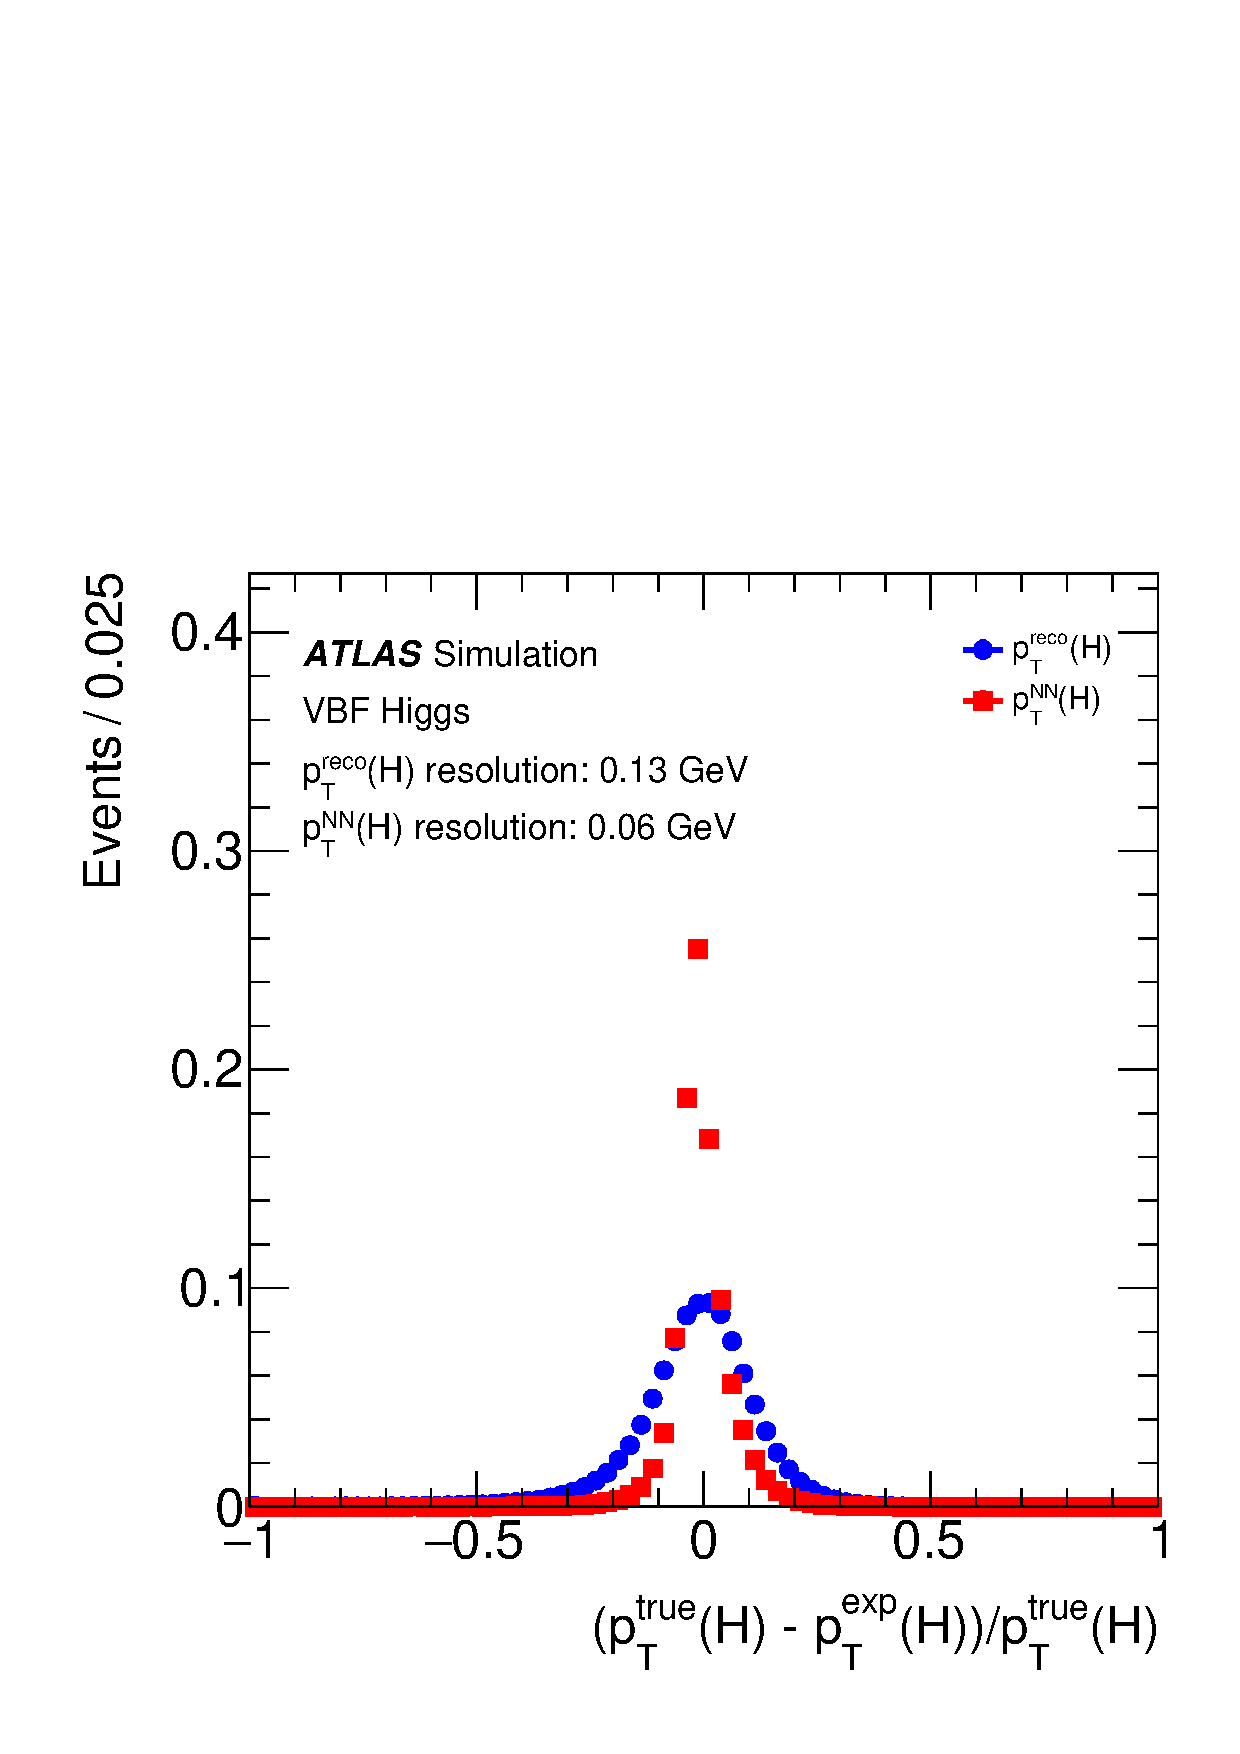
\includegraphics[width=0.55\textwidth]{NN_1.pdf}
    \caption{Resolution of $p_{\text{T}}^{H}$ with respect to truth simulation, comparing the reconstruction from the sum of the $\tau$-lepton four-momenta and \etmiss with the NN-based regression for simulated VBF Higgs boson events~\cite{differential_htautau}.}
    \label{fig:ptH_resolution}
\end{figure}

%%%%%%%%%%%%%%%%%%%%%%%%%%%%%%%%%%%%%%%%%%%%%%%%%%%%%%%%%%%%%%%%%%%%%%%%%%%%%%%%%%%%%%%%%%%%%%%%%%%%%%%%%%%%%%%%%%%%%%%%%%%%%%%%%%%%%%%%%%%%%%%%%%%%%%%%%%%%%%%%%%%%%%%%%%%%%%%%%%%%
\section{Event selection and background definition}
\label{sec:event_selection_background}

The event selection in the \htautau\ analysis can be regarded as a two-stage procedure. 
First, events are divided into three channels according to the decay mode of the $\tau$-leptons, as already defined. 
Subsequently, each channel is further classified into event categories specifically designed to isolate a given Higgs boson production mode considered as signal. 
The goal is to maximize the sensitivity to the Standard Model Higgs boson signal, while ensuring a robust estimation of the Higgs observables reconstructed from the $\tau$-leptons, and to match as closely as possible the phase-space binning defined by the STXS framework.

In the present work, the focus is on the \ttHtt\ process in the fully hadronic channel. 
The selection therefore requires exactly two reconstructed $\tau_{\text{had-vis}}$ objects. 
The transverse-momentum thresholds of these candidates are dictated by the ditau trigger used to collect the events entering the analysis, as explained in Section~\ref{sec:object_definiton}. 
Additional requirements are applied to reduce the trigger rate and to suppress background contributions, particularly at low-$p_{\text{T}}$. 
In particular, the angular separation between the two $\tau_{\text{had-vis}}$ candidates is required to satisfy $\Delta R > 0.6$ in order to avoid overlaps, and at least one additional central jet ($|\eta| < 3.2$) with $p_{\text{T}} > 70$~GeV is required, which reduces the rate contribution from dijet background processes.

Furthermore, the two $\tau_{\text{had-vis}}$ candidates are required to have opposite electric charge. 
Unlike other production modes considered in the \htautau\ analysis, no $b$-jet veto is applied in this channel, since $b$-jets are expected from the top-quark decays accompanying the Higgs boson in \ttH\ production. 
Finally, to enhance the reconstruction efficiency of the invariant mass of the system, additional requirements are imposed on the missing transverse momentum $\met$ and on the visible momentum fractions of the $\tau$-leptons ($x_0$ and $x_1$). 
All selection requirements are summarised in Table~\ref{tab:tth_hadhad_selection}.

\begin{table}[htbp]
    \centering
    \caption{Summary of the event selection for the $\tau_{\text{had}}\tau_{\text{had}}$ channel and the dedicated $t\bar{t}(0\ell)H \to \tau_{\text{had}}\tau_{\text{had}}$ category.}
    \renewcommand{\arraystretch}{1.6} % más espacio vertical
    \scriptsize % letra un poco más pequeña
    \begin{tabular}{l c}
    \hline
    \textbf{Preselection} & $\tau_{\text{had}}\tau_{\text{had}}$ \\
    \hline
    Object counting & \# of $e/\mu = 0$, \# of $\tau_{\text{had-vis}} = 2$ \\
    $p_{\text{T}}$ cut & $\tau_{\text{had-vis}}$: $p_{\text{T}} > 40, 30$~GeV \\
    ID, Isolation, and eveto & $\tau_{\text{had-vis}}$: RNN Medium \\
    Charge product & Opposite charge \\
    Kinematics & -- \\
    $b$-veto & (None in $t\bar{t}(0\ell)H \to \tau_{\text{had}}\tau_{\text{had}}$) \\
    \etmiss & \etmiss $> 20$~GeV \\
    Leading jet & $p_{\text{T}} > 70$~GeV, $|\eta| < 3.2$ \\
    Angular & $0.6 < \Delta R_{\tau_{\text{had-vis}}\tau_{\text{had-vis}}} < 2.5$, 
               $|\Delta\eta_{\tau_{\text{had-vis}}\tau_{\text{had-vis}}}| < 1.5$ \\
    Coll. app. $x_1, x_2$ & $0.1 < x_1 < 1.4$, $0.1 < x_2 < 1.4$ \\
    \hline
    \end{tabular}
    
    \vspace{0.6cm}
    
    \begin{tabular}{l c}
    \hline
    \textbf{Category} & $\tau_{\text{had}}\tau_{\text{had}}$ \\
    \hline
    $t\bar{t}(0\ell)H \to \tau_{\text{had}}\tau_{\text{had}}$ & 
    \# of jets $\geq 6$ and \# of $b$-jets $\geq 1$ \\
    & or \# of jets $\geq 5$ and \# of $b$-jets $\geq 2$ \\
    \hline
    \end{tabular}
    
    \label{tab:tth_hadhad_selection}
    \end{table}
    
The prerequisites described above apply mainly to the $\tauh\tauh$ channel. 
For the \ttH\ production mode under study, the final state is further characterized by the presence of six jets, two of which are expected to be tagged as $b$-jets, as illustrated in Fig.~\ref{fig:tth_topo}. 

To increase the signal acceptance, this selection is slightly relaxed. Events with four or fewer jets are dominated by background, while a significant fraction of the signal appears in events with at least five jets. 
Given the large background contribution observed in events with exactly five jets and only one $b$-jet, the final requirement is defined as either more than five jets with at least two $b$-tags, or more than six jets with at least one $b$-tag.

\begin{figure}[htbp]
    \centering
    \begin{subfigure}[b]{0.48\textwidth}
        \centering
        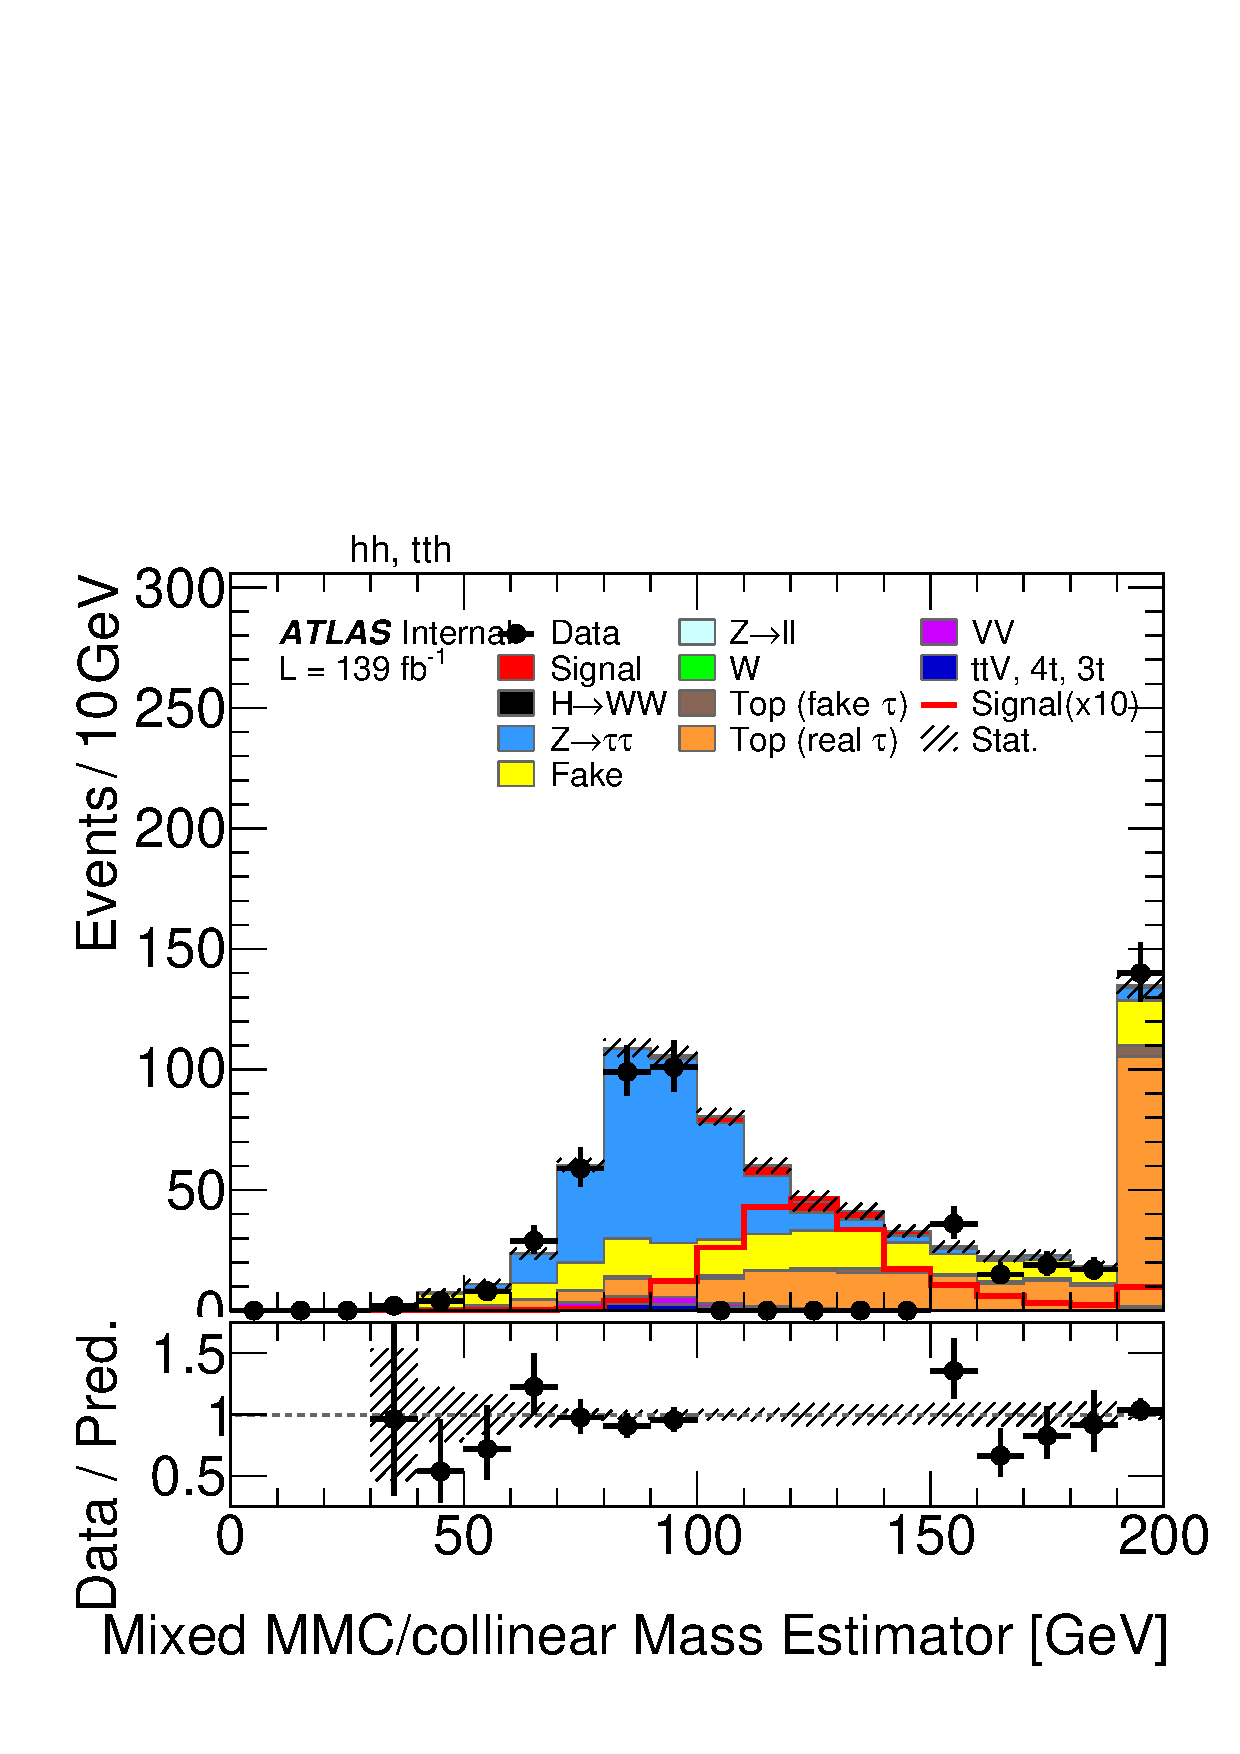
\includegraphics[width=\textwidth]{plot_ditau_mmc_mlm_m_fix_hh_tth.pdf}
        \caption{}
        \label{reconstructed_preselection_a}
    \end{subfigure}
    \hfill
    \begin{subfigure}[b]{0.48\textwidth}
        \centering
        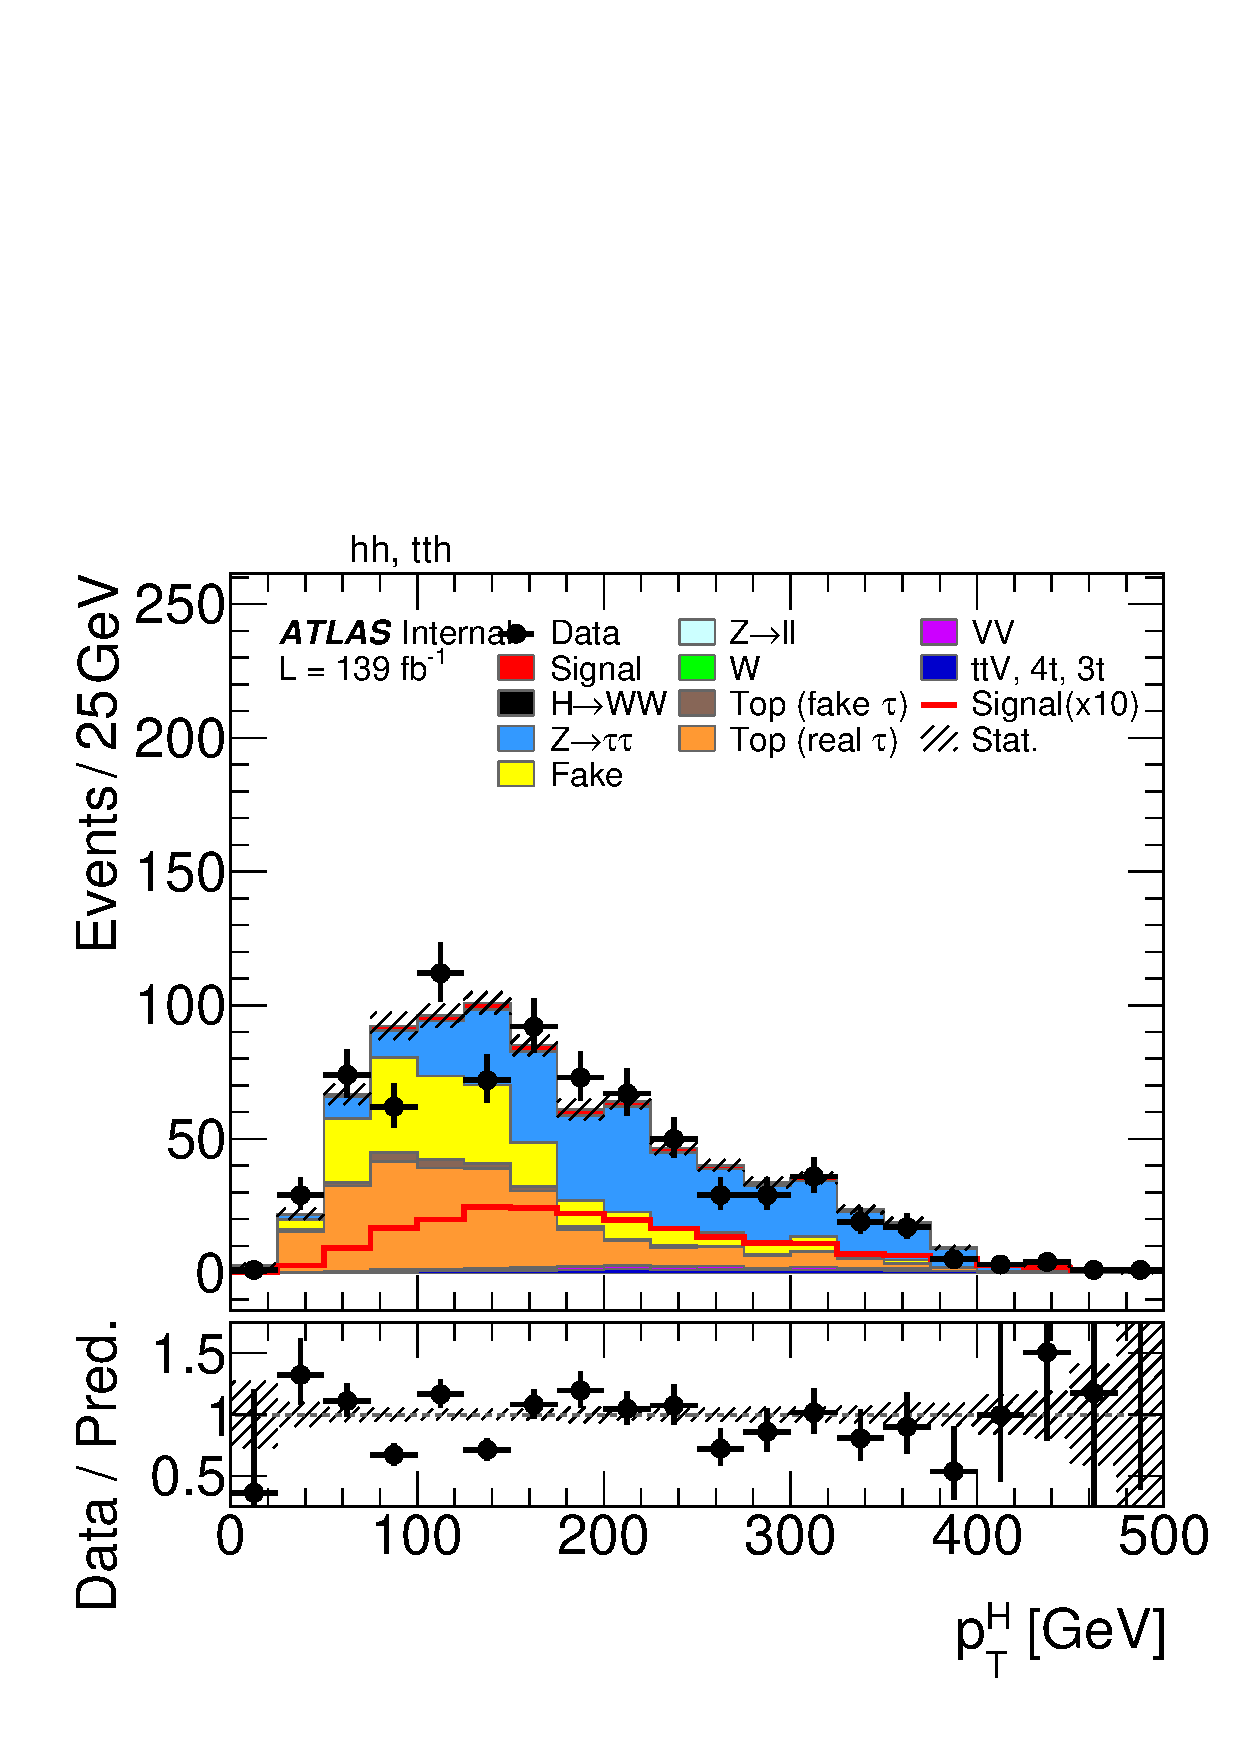
\includegraphics[width=\textwidth]{plot_ditau_pt_NN_kin_hh_tth.pdf}
        \caption{}
        \label{reconstructed_preselection_a}
    \end{subfigure}
    \caption{Distributions of (a) the Higgs boson mass, reconstructed with the mixed MMC/collinear estimator, and (b) the Higgs transverse momentum $p_{\text{T}}^H$, shown at the $t\bar{t}H$ preselection level. Only statistical uncertainties are included.}
    \label{reconstructed_preselection}
\end{figure}


Figure~\ref{reconstructed_preselection} shows the reconstructed Higgs boson candidate mass and \pth distributions in data and MC simulation after applying the preselection. 
From the invariant mass distribution in Fig.~\ref{reconstructed_preselection_a}, the main backgrounds affecting the analysis can be clearly identified. 
Already with this single variable, a first signal-to-background discrimination can be achieved by defining appropriate cuts. 

The dominant background arises from \ztautau$+$jets events, which peak below the Higgs boson signal, around the $Z$ mass of 90~GeV. 
A flatter contribution comes from \ttbar production, since the $\tau$ leptons originate from different particles. 
These events populate the high-mass tail, reflecting the higher energy scale of the process. In addition, a non-negligible contribution is given by QCD multijet events where one or two jets are misidentified as \tauhadvis candidates, referred to as \emph{fakes}. 

After applying the preselection, the expected yields are $309.0 \pm 5.6$ \ztautau events, $266.3 \pm 6.7$ \ttbar events, $184.5 \pm 8.6$ fakes, and $19.5 \pm 0.3$ \ttHtt signal events (all uncertainties statistical only). The \mmc variable therefore allows the definition of three regions with improved signal-to-background ratios:
\begin{itemize}
    \small
    \item Higgs $\mmc$ window ($100~\text{GeV} < \mmc < 150~\text{GeV}$): Signal enhanced region.
    \item High $\mmc$ sideband ($\mmc > 150~\text{GeV}$): Dominated by $t\bar{t}$ events.
    \item Low $\mmc$ sideband ($0 < \mmc < 100~\text{GeV}$): Dominated by $Z(\tau\tau)$ production, since its distribution will peak around the $Z$ boson mass.
\end{itemize}

In practice, the final categorization of events into multiple signal and control regions targeting the different STXS bins is not performed using the \mmc variable, since its distribution is exploited directly in the likelihood fit used to extract the signal, as discussed in Section~\ref{sec:statistical_tth}. 
Instead, dedicated multivariate discriminants are trained to enhance the signal contribution over the backgrounds in specific signal regions and to define control regions that constrain and validate the background components in the final statistical fit. 
Further details on these classifiers are provided in Section~\ref{sec:tth_mva}.  

We now turn to the estimation of the main backgrounds in the \ttHtt analysis. 
The dominant background arises from \ztautau+jets processes, contributing more than $40\%$ of the total background yield. 
These events are modeled with the MC simulations described in Section~\ref{subsec:higgs_mc}, and their modeling and normalization are validated against data in dedicated control regions enriched in this background, defined using the MVA discriminants as detailed in Section~\ref{sec:tth_categories}. 
Similarly, \ttbar production is modeled with MC and validated in data using dedicated control regions within the analysis phase space.  

The third major background contribution comes from fakes, i.e.\ QCD multijet events in which one or two jets are misidentified as \tauhadvis candidates. 
This background is estimated with a data-driven fake-factor (FF) method~\cite{fakes_paper}. 
The contribution of fakes to the signal regions is derived from dedicated control regions, one of which is the anti-ID region, where one of the \tauhadvis candidates fails the Medium working point (WP) but passes the Loose WP, such that the event is still retained in the analysis. 
In this region, a template for the fake contribution is obtained by subtracting simulated prompt-\tauhadvis backgrounds from the data distribution. 
This template is then scaled by a transfer factor, the fake factor (FF), correcting for the different selection efficiencies between pass- and anti-\tauhadvis candidates.  

Two sets of FFs are used, derived in $W$+jets control regions of the \taulephad channel enriched in jets faking \tauhadvis. This choice recycles the work developed in that channel of the \htautau analysis and can be extended to \tauhadhad with the additional consideration of cases where both \tauhadvis are fakes. 
The need for two sets arises because the analysis does not contain events without at least Loose \tauhadvis candidates, so FFs are combined from regions defined with a Loose requirement and from regions without it.  

Since the derivation of FFs relies on \taulephad control regions, the \tauhadvis selection is adjusted to closely match that of the \tauhadhad channel to ensure applicability. The FFs are therefore computed in three distinct regions for the two sets under consideration, differing only in the applied identification requirement. 
In both cases, the numerator is given by the number of data events in the $W$+jets control region with the Medium WP applied, while the denominator corresponds to the anti-\tauhadvis region, defined by inverting the requirement in the not-medium (nm) case, or by requiring at least the Loose WP in the loose-not-medium (lnm) case. 
As before, events with genuine \tauhadvis are subtracted in all regions using MC simulation. 
The resulting FFs, which encapsulate the probability for jets faking \tauhadvis to pass the identification relative to those rejected, are thus defined as:

\begin{align}
    FF_{nm} &= 
    \frac{(\text{Data} - \text{MC})^{\text{WCR}}_{\text{medium } \tau_{\text{had-vis}}}}
         {(\text{Data} - \text{MC})^{\text{WCR}}_{\text{not-medium } \tau_{\text{had-vis}}}}, \nonumber \\[6pt]
    FF_{lnm} &= 
    \frac{(\text{Data} - \text{MC})^{\text{WCR}}_{\text{medium } \tau_{\text{had-vis}}}}
         {(\text{Data} - \text{MC})^{\text{WCR}}_{\text{loose-not-medium } \tau_{\text{had-vis}}}},
\end{align}
where fake factors are derived in bins of \pt and $|\eta|$ of the \tauhadvis candidates, as they exhibit a significant dependence on these variables. 
Ultimately, the smaller the FFs, the better the performance of the \tauhad identification algorithm, since this indicates a lower probability for jets to mimic \tauhadvis candidates.  

The estimation of the fake background is obtained by weighting the \tauhadhad anti-ID events with the corresponding FFs, which provides the predicted number of jets misidentified as \tauhadvis in the signal region. 
The set of regions used for the application of FFs depends on the identification criteria adopted. 
Further details on the FF application can be found in earlier rounds of the \Htautau analysis~\cite{couplings} and in Chapter~\ref{chap:run3_tth}, where a direct contribution was made to the re-estimation of fakes using the reprocessed Run-2 and Run-3 data, including the implementation of new $\tau$-lepton identification techniques.  

Although the full discussion of systematic uncertainties affecting this analysis is deferred to Section~\ref{sec:tth_systematics}, the specific uncertainties associated with the estimation of this background are evaluated through three types of variations. 
The differences observed with respect to the nominal procedure are taken as the systematic uncertainty assigned to the fake background estimate.  

The first group corresponds to the statistical uncertainties of the fake factors derived in the $W+$jets control regions (CRs).  
These are evaluated by varying the fake factors within one standard deviation of their statistical uncertainty, which arises from the limited size of the $W+$jets samples.  
Independent variations are assigned for 1-prong and 3-prong \tauhadvis candidates, and for the \textit{nm} and \textit{lnm} categories, resulting in four separate uncertainties.  

The second group addresses potential differences in the background composition between the regions where the fake factors are measured and those where they are applied.  
Since the relative fractions of light-quark, gluon, and heavy-flavour jets may vary significantly, dedicated control regions enriched in fake $\tau$ candidates are used to evaluate this effect.  
In addition to the nominal \taulephad $W+$jets CR, alternative \tauhadhad regions are considered: one defined by the separation $\Delta\eta(\tauhadvis,\tauhadvis)$ and another based on same-sign events.  
Fake factors are re-derived in these regions, and the full background estimation procedure is repeated to compare the results with the nominal prediction.  

The third group concerns the parametrization strategy of the fake factors.  
To evaluate this effect, fake factors are recalculated in the \tauhadhad same-sign region using coarser binning to ensure sufficient statistics.  
Separate values for leading and subleading \tauhadvis candidates are obtained and then combined to reproduce the nominal parametrization, since the \taulephad $W+$jets CR does not allow them to be distinguished.  
These same-sign fake factors are subsequently applied to the anti-ID region to perform closure tests.  
The $m_{\tau\tau}^{\text{MMC}}$ distribution is used for this purpose, and the ratio of prediction to data is taken as an additional weight on fake events, thereby defining the associated systematic uncertainty.  

Other minor background contributions, such as diboson production and $t\bar{t}+W/Z$, are found to be negligible.  
These are therefore taken directly from simulation, with normalization uncertainties applied.  
Given their very small impact across all the regions considered, the fit cannot meaningfully constrain their normalization, so a conservative treatment is adopted.  
%%%%%%%%%%%%%%%%%%%%%%%%%%%%%%%%%%%%%%%%%%%%%%%%%%%%%%%%%%%%%%%%%%%%%%%%%%%%%%%%%%%%%%%%%%%%%%%%%%%%%%%%%%%%%%%%%%%%%%%%%%%%%%%%%%%%%%%%%%%%%%%%%%%%%%%%%%%%%%%%%%%%%%%%%%%%%%%%%%%%
\section{MVA strategy for \ttHtt}
\label{sec:tth_mva}

%%%%%%%%%%%%%%%%%%%%%%%%%%%%%%%%%%%%%%%%%%%%%%%%%%%%%%%%%%%%%%%%%%%%%%%%%%%%%%%%%%%%%%%%%%%%%%%%%%%%%%%%%%%%%%%%%%%%%%%%%%%%%%%%%%%%%%%%%%%%%%%%%%%%%%%%%%%%%%%%%%%%%%%%%%%%%%%%%%%%
\section{Event categorization}
\label{sec:tth_categories}

%%%%%%%%%%%%%%%%%%%%%%%%%%%%%%%%%%%%%%%%%%%%%%%%%%%%%%%%%%%%%%%%%%%%%%%%%%%%%%%%%%%%%%%%%%%%%%%%%%%%%%%%%%%%%%%%%%%%%%%%%%%%%%%%%%%%%%%%%%%%%%%%%%%%%%%%%%%%%%%%%%%%%%%%%%%%%%%%%%%%
\section{Systematic Uncertainties}
\label{sec:tth_systematics}

%%%%%%%%%%%%%%%%%%%%%%%%%%%%%%%%%%%%%%%%%%%%%%%%%%%%%%%%%%%%%%%%%%%%%%%%%%%%%%%%%%%%%%%%%%%%%%%%%%%%%%%%%%%%%%%%%%%%%%%%%%%%%%%%%%%%%%%%%%%%%%%%%%%%%%%%%%%%%%%%%%%%%%%%%%%%%%%%%%%%
\section{Statistical fit}
\label{sec:statistical_tth}


%From the previous Statistical Methods Chapters, reduced to Machine Learning Techniques

%\section{Statistical Modelling}
%\label{sec:stat_modelling}
% Aquí irán aspectos relacionados con la construcción de modelos estadísticos,
% likelihoods, parámetros, modelado de fondo/señal, etc.

%\section{Statistical Inference}
%\label{sec:stat_inference}
% Aquí se incluirán conceptos sobre estimadores, verosimilitud, p-valores, intervalos de confianza,
% tests de hipótesis, profile likelihood, significancia, etc.


%Statistical techniques play a central role in high-energy physics, as they provide the tools needed to interpret, quantify, and extract meaningful information from the experimental results obtained at the LHC. This chapter outlines the different statistical methods employed throughout this thesis. A frequentist approach is adopted, in which the concept of probability refers to the relative frequency of an outcome in a repeatable experiment.

%First, the statistical modelling of experimental data is introduced, including the construction of the likelihood function for binned data and the treatment of systematic uncertainties through nuisance parameters. This modelling stage provides the essential ingredients subsequently used for the statistical inference, which allow us to extract physics results from the data, including parameter estimation and hypothesis testing. The framework used for building and implementing these statistical models is \textsc{TRExFitter}~\cite{trexfitter}, which relies on the \textsc{HistFactory}~\cite{histfactory} format and the \textsc{RooFit}~\cite{roofit} and \textsc{RooStats}~\cite{roostats} environments for model definition and statistical interpretation.


%%%%%%%%%%%%%%%%%%%%%%%%%%%%%%%%%%%%%%%%%%%%%%%%%%%%%%%%%%%%%%%%%%%%%%%%%%%%%%%%%%%%%%%%%%%%%%%%%%%%%%%%%%%%%%%%%%%%%%%%%%%%%%%%%%%%%%%%%%%%%%%%%%%%%%%%%%%%%%%%%%%%%%%%%%%%%%%%%%%%
\section{STXS results for \ttH}
\label{sec:results_ttH}